\documentclass{scrartcl}

\usepackage{german}
\usepackage[utf8]{inputenc}  %Umlaute
\usepackage[T1]{fontenc}     %Umlauttrennung
\usepackage{lmodern}         %modernes Schriftbild
\usepackage{amsmath}         %math Umgebungen
\usepackage{hyperref}
\usepackage{graphicx}
\usepackage{gensymb}

\title{Physikpraktikum für Naturwissenschaftler \\ Versuch: Drehschwingungen}
\author{Felix Burr, Johannes Spindler (Gruppe 13)}
\date{Durchgeführt am 18. Oktober 2018}


\begin{document}
\begin{titlepage}
  \begin{center}
    \vspace*{1cm}
    \LARGE
    Physikpraktikum für Naturwissenschaftler \\
    \vspace*{1cm}
    \Huge
    \textbf{Versuch: Drehschwingungen} \\
    \vspace*{0.3cm}
    \Large
    Durchgeführt am 18. Oktober 2018 \\
    Betreuer: Christian Ganslmayer \\
    \vspace*{2.5cm}
    Gruppe 13 \\
    Felix Burr: felix.burr@uni-ulm.de \\
    Johannes Spindler: johannes.spindler@uni-ulm.de \\
    \vfill 
  \end{center}
  Wir bestätigen hiermit, das Protokoll selbstständig erarbeitet zu haben und in genauer Kenntnis über dessen Inhalt zu sein. \\
  \vspace*{0.8cm}
  \\
  Felix Burr
  \hfill
  Johannes Spindler
\end{titlepage}
\pagebreak
\tableofcontents


\pagebreak

\section{Einleitung}
Schwingungen sind uns aus vielfachen Alltagssituationen bekannt. Etwa beim Spielen eines Klaviers: Der Ton kommt durch das Schwingen der Saiten zustande und mithilfe der Pedale kann eine Dämpfung der Saitenschwingung eingestellt werden.
Auch in der Architektur müssen mögliche Schwingungen bedacht werden. Erdbeben und Sturm können starke erzwungene Schwingungen an Hochhäusern und Brücken verursachen. Im schlimmsten Fall, einer Resonanz zwischen Anregungs- und Systemfrequenz kommt es zu extremen Auslenkungen und Konstruktionen stürzen womöglich ein.
Deshalb werden wir uns in diesem Versuch mit Drehschwingungen beschäftigen, vor allem mit Dämpfung, erzwungener Schwingung und Resonanz.
\section{Versuch 1: Frequenz und Dämpfung der freien Schwingung}
\subsection{Versuchsdurchführung}
Limilmmlinlina
\subsection{Messwerte und Ergebnisse}

\subsection{Fehlerrechnung}

\subsection{Ergebnisdiskussion}


\section{Versuch 2: Erzwungene Schwingungen}
\subsection{Versuchsdurchführung}
In diesem Versuch wird das Drehpendel von einem externen Motor erregt. Wir untersuchen
wie sich unterschiedliche Erregerfrequenzen auf das Pendel auswirken.

\begin{figure}[h]
  \caption{Drehpendel mit Erreger}
  \centering
    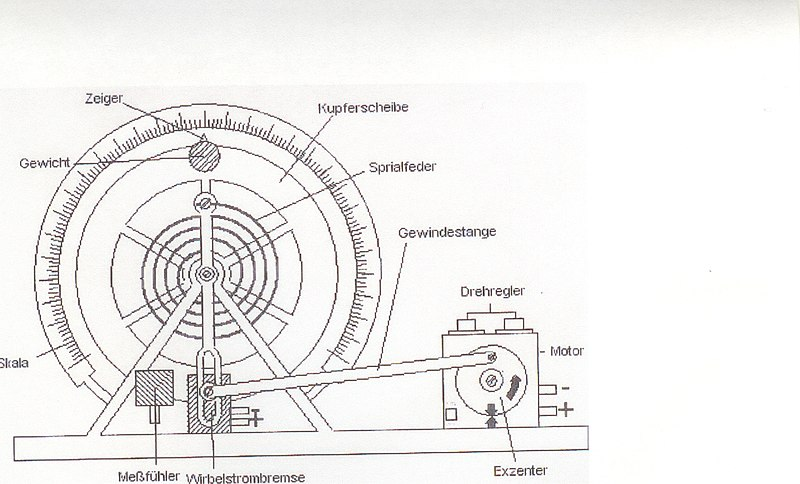
\includegraphics[width=0.75\textwidth]{800px-Pohlsches_Rad}
\end{figure}

In Versuch 2.1 haben wir durch probieren festgestellt, dass der optimale Phasenwinkel bei etwa 105$\degree$ liegt. 
\subsection{Messwerte und Ergebnisse}
Dämpfungsspannung von 2V:\\
\begin{tabular}{llllll}
Messung &F ($\frac{1}{10s}$)&Phasendifferenz ($ms$)&Phasendifferenz ($\degree$)&T ($ms$)&Amplitude ($cm$)\\\hline
1&40&145&24.1&2166&3.5\\
2&42&172&27.9&2216&6.5\\
3&43&295&49.6&2143&11\\
4&44&575&99.2&2086&15.2\\
5&45&945&176.0&1932&6.6\\
6&47&920&178.2&1859&2.9\\\\
\end{tabular}

Dämpfungsspannung von 4V:\\
\begin{tabular}{llllll}
Messung &F ($\frac{1}{10s}$)&Phasendifferenz ($ms$)&Phasendifferenz ($\degree$)&T ($ms$)&Amplitude ($cm$)\\\hline
1&40&312&51.8&2167&2.7\\
2&42&428&74.3&2073&3.9\\
3&43&523&93.0&2025&4.6\\
4&44&575&99.2&2086&15.2\\
5&45&625&113.5&1982&4\\
\end{tabular}
\subsection{Fehlerrechnung}

\subsection{Ergebnisdiskussion}


\section{Versuch 3: Computersimulation}
\subsection{Versuchsdurchführung}

\subsection{Messwerte und Ergebnisse}

\subsection{Fehlerrechnung}

\subsection{Ergebnisdiskussion}

\end{document}
